

\section{Warum ist die Erde nicht flach?}

\begin{figure}
	\begin{center}
		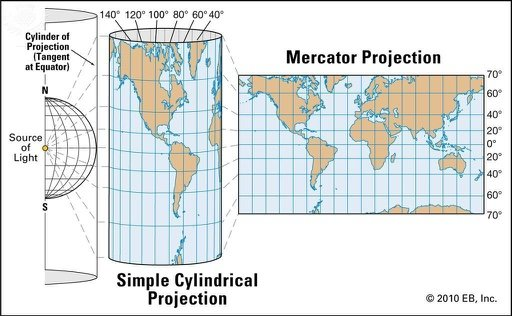
\includegraphics[width=10cm]{papers/nav/bilder/projektion.png}
		\caption[Mercator Projektion]{Mercator Projektion}
	\end{center}	
\end{figure}

Es gibt heutzutage viele Beweise dafür, dass die Erde eine Kugel ist. 
Die Fotos von unserem	Planeten oder die Berichte der Astronauten. 
Aber schon vor ca. 2300 Jahren hat Aristoteles bemerkt, dass Schiffe im Horizont verschwinden und die einzige Erklärung dafür die Kugelgestalt der Erde ist.
Auch der Erdschatten bei einer Mondfinsternis ist immer rund.
Eratosthenes konnte etwa 100 Jahre später den Erdumfang berechnen. 
Er beobachtete, dass die Sonne in Syene mittags im Zenit steht und gleichzeitig in Alexandria unter einem Winkel einfällt. 
Mithilfe der Trigonometrie konnte er mit dem Abstand der Städte und dem Einfallswinkel den Umfang berechnen.

Der Kartograph Gerhard Mercator projizierte die Erdkugel auf ein Papier und erstellte so eine winkeltreue Karte. 
Jedoch wurden die Länder, die einen grösseren Abstand zum Äquator haben vergrössert, damit die Winkel stimmen können. 
Wurde man also nun davon ausgehen, dass die Erde flach ist so würden wir nie dort ankommen wo wir es wollen.

Dies sieht man zum Beispiel sehr gut, wenn man die Anwendung Google Earth und eine Weltkarte vergleicht. 
Grönland ist auf der Weltkarte so gross wie Afrika. 
In der Anwendung Google Earth jedoch ist Grönland etwa so gross wie Algerien. 
Das liegt daran, das man die 3D – Weltkarte nicht einfach auslegen kann. 

